\chapter{Two Dimensions and Other Exact Models}\label{ch:twod}

Chapter~\ref{ch:hitting} ended with methods that learn the gap from samples. Those methods are tested, and the theory behind them is calibrated, on the worlds where everything can be computed. This chapter collects them: two dimensional Yang Mills theory, where the gap is a statement about Brownian motion on a compact group (Section~\ref{sec:su2bm}) and a guided tour of the whole method in that case (Section~\ref{ch:tour}); Riemann's kernel on the three sphere (Section~\ref{ch:riemann}); dynamic and static gaps (Section~\ref{ch:dynamic}); the renormalization group (Section~\ref{ch:rg}); free fields (Section~\ref{ch:freefield}); and large $N$ (Section~\ref{ch:largeN}). None of them is four dimensional Yang Mills. Each shows what an exact answer looks like, and the chapters on the ladder put back what is missing.

\section{Brownian Motion on SU(2)}\label{sec:su2bm}

In two dimensions Yang Mills theory can be solved exactly, on the lattice~\cite{Mi75} and in the continuum~\cite{GKS89,Se97,Le03}, and the solution is a statement about Brownian motion\index{Brownian motion on SU(2)} on a compact group. This section works out that statement for SU(2) and proves the uniform Thorin gap inequality of Section~\ref{ch:routeB} from the coarsest lattice all the way to the continuum.

\subsection{Brownian motion on the three sphere}

The group SU(2) consists of matrices $\begin{pmatrix}a&-\bar b\\ b&\bar a\end{pmatrix}$ with $|a|^2+|b|^2=1$, so it is the unit sphere $S^3\subset\mathbb C^2$. Every element is conjugate to $\operatorname{diag}(e^{i\theta},e^{-i\theta})$ for a unique rotation angle $\theta\in[0,\pi]$, which is the geodesic distance from the identity. Class functions depend only on $\theta$, and the Haar measure\index{Haar measure} pushes forward to the density $\frac2\pi\sin^2\theta$ on $[0,\pi]$.

The irreducible representations are indexed by their dimension $n=1,2,3,\dots$, with characters
\[
\chi_n(\theta)=\frac{\sin n\theta}{\sin\theta}
\]
and Casimir\index{Casimir} eigenvalues $(n^2-1)/4$. With the Laplacian normalised so that these are the eigenvalues, Brownian motion on SU(2) started at the identity has, at time $t$, the density with respect to Haar measure
\[
K_t(\theta)=\sum_{n\ge1}n\,e^{-t(n^2-1)/4}\,\chi_n(\theta).
\]
Three readings of this formula will be used repeatedly.
\begin{enumerate}
\item[(i)] The character coefficients $u_n(t)=e^{-t(n^2-1)/4}$ are the Fourier transform of the law of the Brownian position, and the Casimir is its Laplace exponent. Convolution of laws multiplies Fourier coefficients, so $K_t*K_{t'}=K_{t+t'}$: Brownian times add.
\item[(ii)] The smallest nonzero Laplace exponent is $3/4$. It is the spectral gap of the Laplacian on $S^3$ in this normalisation, and the exponential rate at which Brownian motion on SU(2) forgets its starting point and approaches the Haar law.
\item[(iii)] For small $t$, Poisson resummation gives the image sum
\[
K_t(\theta)\propto t^{-3/2}e^{t/4}\sum_{m\in\Z}\frac{\theta+2\pi m}{\sin\theta}\,e^{-(\theta+2\pi m)^2/t},
\]
dominated by $m=0$: $K_t(\theta)\approx c\,t^{-3/2}\,\frac{\theta}{\sin\theta}\,e^{-\theta^2/t}$. The factor $\theta/\sin\theta$ is $j^{-1/2}$, the inverse square root of the Jacobian $j=(\sin\theta/\theta)^2$ of the exponential map (Section~\ref{sec:jacobian}). It is the only trace of curvature at short times, and it will carry asymptotic freedom\index{asymptotic freedom} in Section~\ref{ch:mk}.
\end{enumerate}

\begin{figure}[t]
\centering
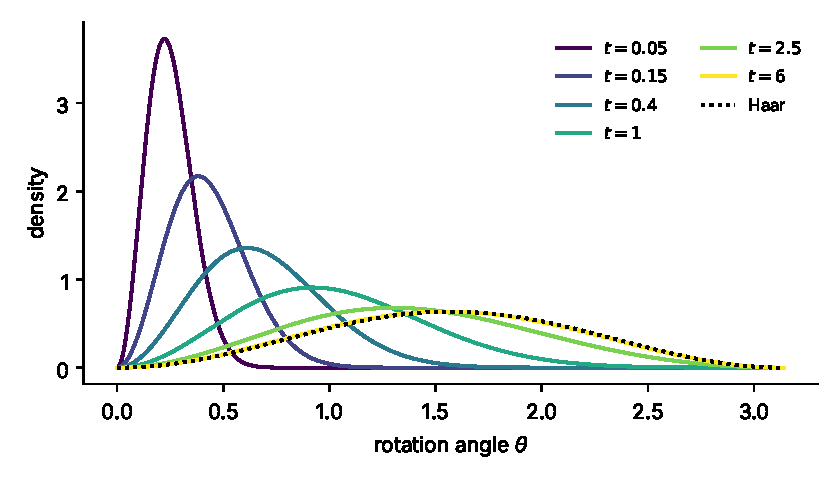
\includegraphics[width=0.92\textwidth]{figures/heat_kernel_laws.pdf}
\caption[Laws of the rotation angle of Brownian motion on SU(2) at several times, against the Haar law]{Laws of the rotation angle of Brownian motion on SU(2) at several times, against the Haar law. At small times the law is a three dimensional Gaussian in disguise; at large times it relaxes to Haar at the rate $3/4$ set by the first Casimir.}
\label{fig:hklaws}
\end{figure}

\subsection{The continuum theory on a surface}

Migdal~\cite{Mi75} discovered, and Witten~\cite{Wi91} later explained in geometric terms, that two dimensional Yang Mills theory on a closed surface $\Sigma$ of genus $h$ and area $A$ has partition function
\[
Z_h(A)=\sum_R(\dim R)^{2-2h}\,e^{-A\,C_2(R)/2},
\]
with the coupling absorbed into the area. For SU(2) this is
\[
Z_h(A)=\sum_{n\ge1}n^{2-2h}\,e^{-A(n^2-1)/8}.
\]
The theory has no local degrees of freedom; its only invariant is the area (the normalisation of $Z_h$ is fixed only up to a factor $e^{cA}$~\cite{Wi91}; rigorous constructions are in~\cite{Se97,Le03}). For every genus the partition function is completely monotone in $A$, since all the weights $n^{2-2h}$ are positive, with spectral measure\index{spectral measure} $\sum_{n\ge2}n^{2-2h}\delta_{(n^2-1)/8}$ after the trivial representation is removed. Area plays the role of Euclidean time, and the gap is $3/8$. Theorem~\ref{thm:rateB} applies verbatim with area in place of time (Figure~\ref{fig:2dgapB}).

The Route B Thorin density\index{Thorin density} has an especially clean form here. On the torus it is $\psi_A(y)/(\pi y)$, where $\psi_A(y)=Z(A)-\operatorname{Re}Z(A+iy)$ with the vacuum removed, and $Z(A+iy)$ is a Jacobi theta function at complex modulus. It is periodic in the real time $y$, with period $16\pi$, because $n^2-1$ is an integer.

\begin{figure}[t]
\centering
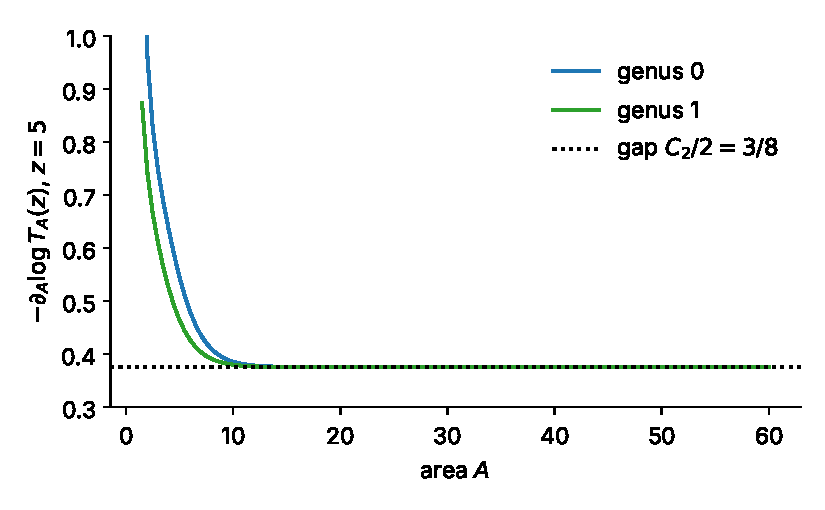
\includegraphics[width=0.8\textwidth]{figures/ym2d_gap.pdf}
\caption[Two dimensional SU(2) Yang Mills on the sphere and the torus: the local Thorin decay rate in area]{Two dimensional SU(2) Yang Mills on the sphere and the torus: the local Thorin decay rate in area converges to the Casimir gap $3/8$.}
\label{fig:2dgapB}
\end{figure}

\subsection{The lattice theory and exact decimation}

On the lattice the key fact is that decimation\index{decimation} is exact in two dimensions. Gluing two adjacent plaquettes along a common link and integrating out that link convolves their weights as class functions. In character variables this multiplies the coefficients:
\[
(f*g)\;\longleftrightarrow\;u_n(f)\,u_n(g).
\]
A block of $b\times b$ plaquettes therefore has weight with coefficients $u_n^{\,b^2}$. For the heat kernel\index{heat kernel} action, $u_n^{b^2}=e^{-b^2t(n^2-1)/4}$, which is again a heat kernel with $t$ multiplied by $b^2$. The heat kernel action is the fixed form of exact decimation, and the parameter $t$ is the area measured in units of the coupling.

Place the theory on a cylinder whose spatial circle has $L$ sites and physical length $\ell$, so the lattice spacing is $a=\ell/L$. For SU(2) the Wilson coupling is $\beta=4/(g^2a^2)$. Physical states are class functions of the holonomy around the circle, and one time step glues a ring of $L$ plaquettes. The transfer matrix\index{transfer matrix} is therefore diagonal in characters, with eigenvalues $u_n(\beta)^L$ where $u_n=I_n/I_1$. In physical units the gauge invariant spectrum is
\[
E_n(a)=-\frac{L}{a}\log u_n(\beta)=-\frac{g^2\ell\beta}{4}\log u_n(\beta),\qquad n\ge1,
\]
with $E_1=0$ the vacuum. Because $I_\nu(\beta)$ decreases in $\nu$, the gap of the whole theory is $\Delta(a)=E_2(a)$. As $a\to0$ the Bessel asymptotics give $u_n=1-(n^2-1)/(2\beta)+O(\beta^{-2})$, so $E_n\to\frac{g^2\ell}{2}\cdot\frac{n^2-1}{4}$, the Casimir spectrum, with continuum gap
\[
\Delta_{\mathrm{cont}}=\frac{3g^2\ell}{8}.
\]
The gap grows linearly with the length of the circle. That is confinement\index{confinement}: the energy of a flux tube wrapping the circle grows with its length. In two dimensions there are no propagating gluons, so this gap is a string tension rather than a particle mass. The point of the exercise is not the physics of two dimensions but the mechanism of the proof, which we now give.

\subsection{A uniform gap from a Bessel inequality}

\begin{lemma}[Bessel ratio bound]\label{lem:amosB}
For all $\beta>0$, $-\log u_2(\beta)\ge\operatorname{arcsinh}\big(\tfrac{3}{2\beta}\big)$.
\end{lemma}

\begin{proof}
Amos\index{Amos, D. E.}'s inequality~\cite{Am74}, valid for $\nu\ge0$, $I_{\nu+1}(\beta)/I_\nu(\beta)\le\beta/\big(\nu+\frac12+\sqrt{\beta^2+(\nu+\frac12)^2}\big)$ at $\nu=1$ gives $u_2\le\beta/\big(\frac32+\sqrt{\beta^2+\frac94}\big)$. With $x=3/(2\beta)$ the right side is $1/(x+\sqrt{1+x^2})=e^{-\operatorname{arcsinh}x}$. We also checked the bound numerically on $[10^{-3},10^4]$.
\end{proof}

\begin{theorem}[two dimensional uniform gap]\label{thm:2dB}
Let $x=3g^2a^2/8$. For every lattice spacing,
\[
\Delta(a)\ \ge\ \Delta_{\mathrm{cont}}\,\frac{\operatorname{arcsinh}x}{x}.
\]
Consequently, for all $L\ge1$ and every gauge invariant observable, the uniform Thorin gap inequality holds in physical units with $K=1$ and
\[
\Delta_0=\Delta_{\mathrm{cont}}\,\frac{\operatorname{arcsinh}x_\ell}{x_\ell},\qquad x_\ell=\tfrac38g^2\ell^2 .
\]
\end{theorem}

\begin{proof}
By Lemma~\ref{lem:amosB}, $\Delta(a)=\frac{g^2\ell\beta}{4}(-\log u_2)\ge\frac{g^2\ell\beta}{4}\operatorname{arcsinh}\frac{3}{2\beta}$. Since $\frac{3}{2\beta}=x$ and $\frac{g^2\ell\beta}{4}=\Delta_{\mathrm{cont}}/x$, this is the stated bound. The function $\operatorname{arcsinh}(x)/x$ decreases on $(0,\infty)$, because $\operatorname{arcsinh}$ is concave and vanishes at the origin, so the bound at the coarsest spacing $a=\ell$ holds for every finer spacing. Theorem~\ref{thm:equivB} converts the uniform spectral gap into the uniform Thorin gap inequality with $K=1$.
\end{proof}

\begin{figure}[t]
\centering
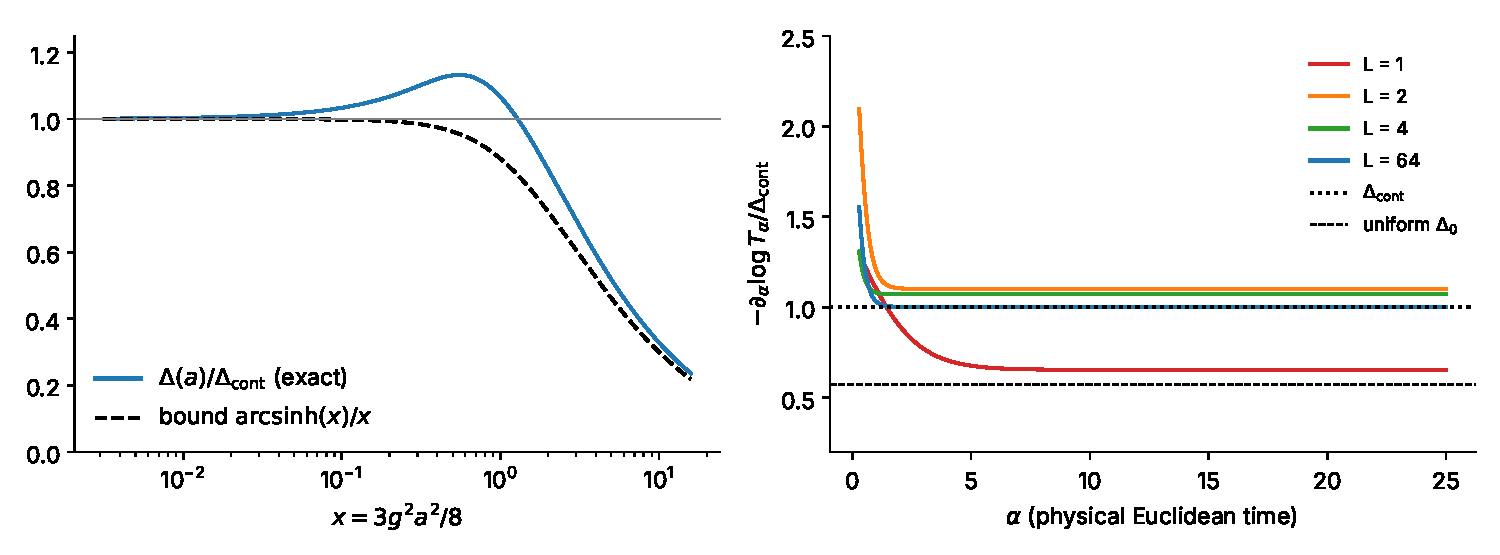
\includegraphics[width=\textwidth]{figures/op1_2d_uniform.pdf}
\caption[Left: the exact lattice gap in units of the continuum gap, against the bound]{Left: the exact lattice gap in units of the continuum gap, against the bound $\operatorname{arcsinh}(x)/x$ of Theorem~\ref{thm:2dB}. The exact ratio overshoots $1$, with a maximum of about $1.13$ near $x\approx0.55$, so the approach to the continuum is not monotone, while the bound is. Right: Thorin local rates in physical units for $L=1,2,4,64$ at $\ell=3$ and $g=1$, all above the uniform $\Delta_0$, the curves for large $L$ approaching $\Delta_{\mathrm{cont}}$.}
\label{fig:2duniformB}
\end{figure}

\subsection{The anatomy of the proof}

The proof has three ingredients, and it is worth naming them because the rest of the book tries to reproduce each in four dimensions.
\begin{enumerate}
\item[(i)] Exact decimation. Coarse graining is a convolution of laws, diagonal in characters, so the transfer matrix eigenvalue is an explicit function of the coupling.
\item[(ii)] A special function inequality. The Bessel ratio bound controls the eigenvalue at every coupling, from strong to weak, and scales like $a^2$ at weak coupling, which exactly cancels the conversion to physical units.
\item[(iii)] The equivalence theorem. A uniform spectral gap is a uniform Thorin gap inequality with constant one.
\end{enumerate}
In four dimensions, ingredient (iii) is available unchanged. Ingredient (i) fails: coarse graining on $\Z^4$ is not a convolution of plaquette laws. The Migdal Kadanoff\index{Migdal Kadanoff recursion} recursion of Section~\ref{ch:mk} restores it at the price of an approximation, by combining convolution with a Bayesian product. Ingredient (ii) becomes the decrement inequality of Section~\ref{ch:verification}.

\section{A Guided Tour in Two Dimensions}\label{ch:tour}\index{two dimensions}\index{decimation}

Two dimensional SU(2) lattice gauge theory is the one case in which every object of this book can be written down and computed in a line. This section walks through the whole argument there, with numbers, as a map of the method. Nothing in it is new. The table and Figure~\ref{fig:tour2d} are exact and are produced by \texttt{code/tour2d.py}; the only Monte Carlo numbers are the ones quoted under Computation, which are checked against exact answers.

\subsection{The measure and its plaquette law}

In two dimensions on the plane, after gauge fixing on a tree, the plaquette variables are independent, each with the Wilson law $e^{\beta\cos\theta}$ times the Haar density $\frac2\pi\sin^2\theta$ on the rotation angle. The normalised character coefficients are ratios of Bessel functions, $u_n=I_n(\beta)/I_1(\beta)$, and the mean plaquette is $u_2$.

\begin{center}
\small
\begin{tabular}{cccccc}
\toprule
$\beta$ & $u_2$ & $u_3$ & $-\log u_2$ & gap ratio & bound \\ \midrule
0.5 & 0.124 & 0.010 & 2.090 & 0.697 & 0.606 \\
1 & 0.240 & 0.039 & 1.426 & 0.951 & 0.797 \\
2 & 0.433 & 0.134 & 0.837 & 1.116 & 0.924 \\
4 & 0.658 & 0.342 & 0.418 & 1.116 & 0.978 \\
8 & 0.819 & 0.590 & 0.199 & 1.063 & 0.994 \\
16 & 0.908 & 0.773 & 0.097 & 1.032 & 0.999 \\
32 & 0.954 & 0.881 & 0.048 & 1.016 & 1.000 \\
\bottomrule
\end{tabular}
\end{center}

\begin{figure}[t]
\centering
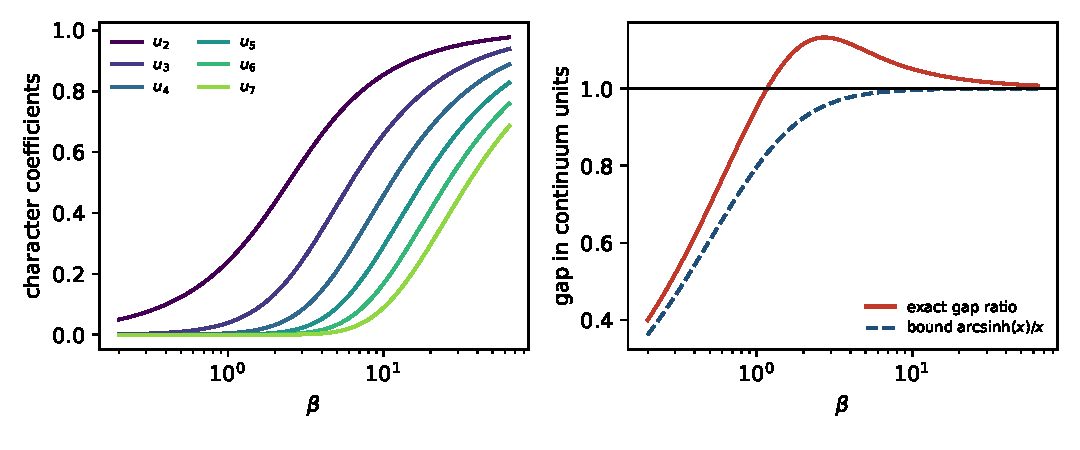
\includegraphics[width=\textwidth]{figures/tour2d.pdf}
\caption[Two dimensional SU(2) at a glance]{Left: the character coefficients $u_n=I_n(\beta)/I_1(\beta)$ of the Wilson plaquette law, $n=2,\dots,7$. Right: the exact lattice gap in units of the continuum gap, and the lower bound from Amos's inequality.}
\label{fig:tour2d}
\end{figure}

Figure~\ref{fig:tour2d} shows the coefficients and the gap across four decades of coupling.

\subsection{Positivity and the spectral measure}

The transfer matrix acts on class functions and is diagonal in the characters, with eigenvalues proportional to $u_n$. Reflection positivity is the statement that these eigenvalues are positive, which is the positivity of the Bessel functions. The spectral measure of a class function observable is a sum of point masses at the energies $E_n=-\log u_n$ in lattice units, and the gap is $E_2=-\log u_2$, the fourth column of the table. The same number is the string tension in lattice units: in two dimensions the Wilson loop of area $A$ is exactly $u_2^A$.

\subsection{The two routes}

Route A: the correlation $\sum_nc_ne^{-E_n\tau}$ with $c_n\ge0$ is the Laplace transform of a positive measure with atoms at the $E_n$; after an offset it is the Thorin measure of a convolution of gamma variables, and the gap is the smallest rate. Route B: the $2\sin^2$ lemma turns the same measure into the Thorin density $T_\alpha(z)=\sum_nc_ne^{-\alpha E_n}\,2\sin^2(E_ny/2)/(\pi y)$ with $y=\sqrt{2z}$, a sum of positive oscillations whose amplitudes decay in $\alpha$ at the rates $E_n$. The slowest is $E_2$.

\subsection{The uniform bound}

The fifth column is the lattice gap in units of the continuum gap, $(-\log u_2)/x$ with $x=3/(2\beta)$, and the sixth is the bound $\operatorname{arcsinh}(x)/x$ of Theorem~\ref{thm:2dB}, which follows from Amos's inequality for Bessel ratios. The bound holds in every row. The gap ratio overshoots one at intermediate coupling and returns to it from above in the continuum limit. A uniform Thorin gap inequality therefore holds from the coarsest lattice to the continuum, which is the conjecture of Section~\ref{ch:isthere} in a case where it is a theorem.

\subsection{Renormalization}

Decimation by a scale factor $b$ is exact in two dimensions (Section~\ref{sec:su2bm}): character coefficients are raised to the power $b^2$, $u_n\mapsto u_n^{b^2}$. In two dimensions bond moving has power $b^{d-2}=1$ and does nothing, so the Migdal Kadanoff ladder is the exact renormalization group, and the two caricatures of Chapter~\ref{ch:sandwich} both coincide with the truth. The width of the bracket in $d$ dimensions is governed by the bond moving power $b^{d-2}$: one in two dimensions, $b$ in three, $b^2$ in four. In the ladder, dimension enters through that exponent alone.

In the heat kernel family, $u_n=e^{-(n^2-1)t/4}$, decimation is $t\mapsto b^2t$: the coupling $\beta=2/t$ is divided by $b^2$ at every step. The coupling is relevant, the flow reaches strong coupling after $\frac12\log_b\beta$ steps, and the gap in physical units is constant along the flow. There is no asymptotic freedom to prove and no crossover to control.

\subsection{Approach to Haar measure}

By the Fourier bound of Section~\ref{ch:h6}, the law of a block of $m$ plaquettes is within $\frac12\big(\sum_{n\ge2}n^2u_n^{2m}\big)^{1/2}$ of Haar measure in total variation. With $m=4$ this is $0.003$ at $\beta=1$, $0.035$ at $\beta=2$ and $0.19$ at $\beta=4$. Confinement in two dimensions is Poincar\'e's shuffle: enough independent group elements multiplied together are uniformly distributed.

\subsection{Computation}

The Monte Carlo estimators of Chapters~\ref{ch:estimation} and~\ref{ch:kac} reported below were tested here against exact answers. On a $3\times3$ torus, $\log Z(2)=-13.8223$ from the character formula; over three seeds the root mean square errors are $0.032$ for the vertical likelihood family, $0.057$ for path sampling (the power posterior), $0.117$ for prior importance sampling, $0.140$ for split sampling, $0.218$ for nested sampling and $0.275$ for the harmonic mean estimator, whose error changes sign across seeds. Pseudolikelihood recovers $\beta$ from one configuration of a $12\times12$ torus to about $15$ percent at $\beta\le2$ and about $5$ percent at $\beta\ge4$. The heat bath is a slice sampler on the three sphere, and Conjecture~\ref{prop:slicecurv}, whose proof is only sketched (the smoothing of the corners of the slice is not carried out), would give its sliced conditional a log Sobolev constant of two, under the positivity hypothesis of that conjecture on every slice level.

\subsection{What two dimensions does not teach}

Three things are absent. There is no bond moving, so no nonlinearity in the renormalization map and no need for the likelihood ratio order. There is no marginal coupling, so no first passage time and no exponentially small scale. And there are no glueballs: the spectrum is that of a single quantum mechanical particle on the group, not of a field theory with propagating degrees of freedom. The rest of the book is about putting those three things back.

\section{Riemann's Kernel and the Three Sphere}\label{ch:riemann}

This section records an identity that connects the two problems of our research programme. Riemann's kernel $\Phi$, whose Fourier transform is the function $\Xi$ of the Riemann Hypothesis\index{Riemann Hypothesis}, is built from the return density of Brownian motion\index{Brownian motion on SU(2)} on SU(2), which is also the partition function of two dimensional Yang Mills theory on the sphere.

\subsection{Riemann's kernel}

Riemann's 1859 memoir~\cite{Ri59} writes the completed zeta function, evaluated on the critical line, as a cosine transform. With
\[
\Phi(u)=\sum_{n\ge1}\big(2\pi^2n^4e^{9u/2}-3\pi n^2e^{5u/2}\big)\exp\big(-\pi n^2e^{2u}\big),
\]
one has
\[
\Xi(x)=4\int_0^\infty\Phi(u)\cos(xu)\,\mathrm du,
\]
where $\Xi(x)=\xi(\tfrac12+ix)$. The kernel $\Phi$ is positive, even, and decays like a double exponential. P\'olya~\cite{Po26} studied the zeros of transforms of this kind; de Bruijn~\cite{dB50} and Newman~\cite{Ne76} studied the deformation $\int e^{\lambda u^2}\Phi(u)\cos(xu)\mathrm du$, which is a backward heat flow on $\Xi$; and the Riemann Hypothesis is the statement that all zeros of $\Xi$ are real. In our Riemann programme $\Phi$, normalised, is the starting point of the probabilistic constructions.

\subsection{The return density of Brownian motion on SU(2)}

The density of Brownian motion on SU(2) at the identity is the heat kernel\index{heat kernel} at $\theta=0$. Since $\chi_n(0)=n$,
\[
K_t(e)=\sum_{n\ge1}n^2e^{-t(n^2-1)/4}.
\]
The partition function of two dimensional SU(2) Yang Mills theory on the sphere is $Z_0(A)=\sum_nn^2e^{-A(n^2-1)/8}$, so
\[
Z_0(A)=K_{A/2}(e):
\]
the sphere partition function at area $A$ is the probability density that Brownian motion on the three sphere, run for time $A/2$, returns to its starting point. This is the probabilistic content of Witten's observation that the sphere partition function is a heat kernel evaluated at the identity.

\subsection{The identity}

\begin{proposition}\label{prop:riemannB}
Let $F(A)=\sum_{n\ge1}n^2e^{-An^2/8}=e^{-A/8}Z_0(A)$. With $A=8\pi e^{2u}$,
\[
\Phi(u)=-16\pi^2e^{9u/2}F'(A)-3\pi e^{5u/2}F(A).
\]
\end{proposition}

\begin{proof}
At $A=8\pi e^{2u}$ we have $e^{-An^2/8}=e^{-\pi n^2e^{2u}}$, and differentiating gives $\sum_nn^4e^{-An^2/8}=-8F'(A)$. Substituting into the definition of $\Phi$ gives the formula.
\end{proof}

So Riemann's kernel is a linear combination, with coefficients depending on $u$, of the return density of Brownian motion on the three sphere and its time derivative, evaluated at time $t=A/2=4\pi e^{2u}$. The derivative has a physical meaning of its own: $-\partial_A\log Z_0$ is the expected action per unit area in two dimensional Yang Mills on the sphere. We checked the identity numerically to fifteen digits (Figure~\ref{fig:riemannB}).

\begin{figure}[t]
\centering
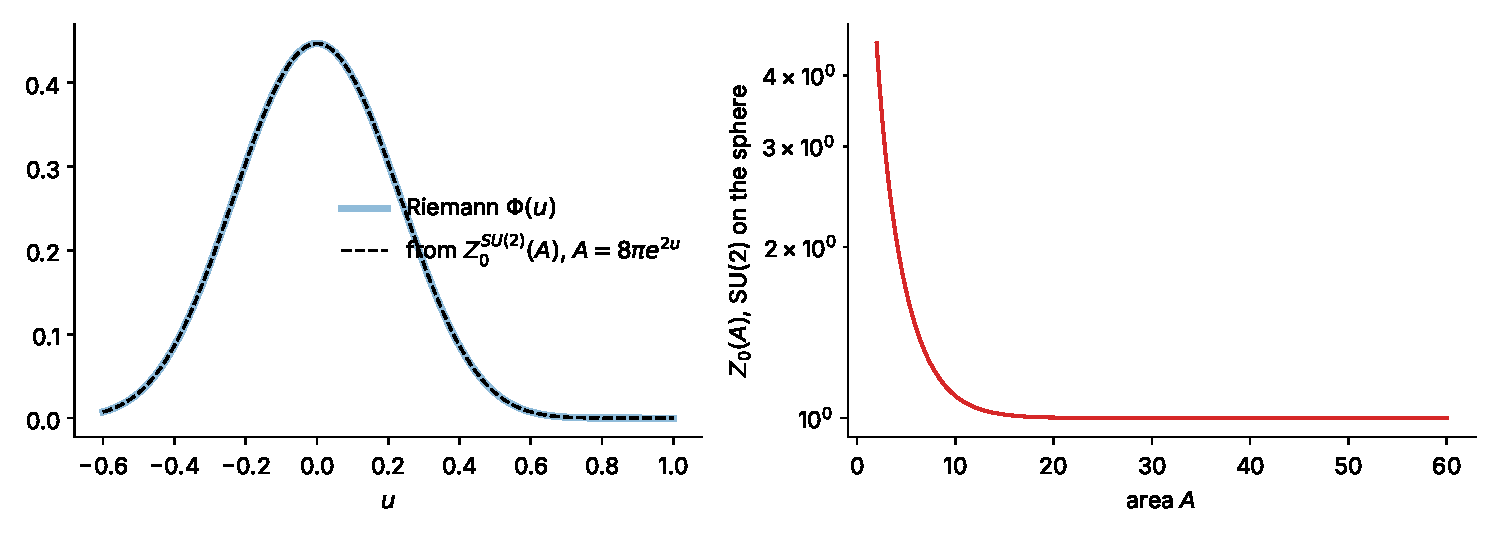
\includegraphics[width=\textwidth]{figures/riemann_kernel_ym.pdf}
\caption[Left: Riemann's $\Phi(u)$ and the same function built from the SU(2) sphere partition function at]{Left: Riemann's $\Phi(u)$ and the same function built from the SU(2) sphere partition function at $A=8\pi e^{2u}$. Right: the sphere partition function $Z_0(A)$, the return density of Brownian motion on $S^3$ at time $A/2$.}
\label{fig:riemannB}
\end{figure}

\subsection{The functional equation as an area duality}

Riemann's functional equation $\xi(s)=\xi(1-s)$ is equivalent to the evenness $\Phi(u)=\Phi(-u)$. Under the identity, $u\mapsto-u$ sends $A=8\pi e^{2u}$ to $8\pi e^{-2u}=64\pi^2/A$. The functional equation therefore becomes a relation between the sphere theory at area $A$ and at area $64\pi^2/A$. On the Yang Mills side this is the Poisson resummation that turns the sum over representations into a sum over classical solutions, the instanton expansion of two dimensional Yang Mills. On the Brownian side it is the relation between the spectral sum and the image sum of Section~\ref{sec:su2bm}: small times on one side correspond to large times on the other.

\subsection{The Biane, Pitman and Yor connection}

The same theta sums appear in the work of Biane, Pitman and Yor~\cite{BPY} on laws tied to Brownian excursions and Bessel bridges. They show that $\xi$ is, up to normalisation, the Mellin transform of a probability law built from these sums, and that the hyperbolic laws $C$, $S_{\mathrm{BPY}}$ and $T$ of Section~\ref{ch:toolkit} are the natural Laplace transform companions. Proposition~\ref{prop:riemannB} adds a gauge theoretic face to that picture: the Mellin side lives on the real line of $\log$ area, the Laplace side lives on Brownian time on SU(2), and the same function is the partition function of a gauge theory.

The variable $S_{\mathrm{BPY}}$, whose Laplace transform is $\sqrt{2q}/\sinh\sqrt{2q}$, will reappear in Section~\ref{ch:mk} for a different reason: that Laplace transform is the curvature factor $\theta/\sin\theta$ at the imaginary angle $\theta=i\sqrt{2q}$, and the mean of $S_{\mathrm{BPY}}$ controls asymptotic freedom\index{asymptotic freedom} in the Migdal Kadanoff ladder. The three sphere thus ties together Riemann's kernel, two dimensional Yang Mills, and the running of the coupling in the ladder.

\subsection{Questions}

\begin{problem}\label{op:exact1}
Study the zeros of $Z_0(A)$ in the complex area plane, the Fisher zeros of the sphere theory, and relate them through Proposition~\ref{prop:riemannB} to the zeros of $\Xi$.
\end{problem}

\begin{problem}\label{op:exact2}
The large $N$ limit of two dimensional Yang Mills on the sphere has a third order phase transition at a critical area, discovered by Douglas and Kazakov\index{Douglas, M. R.!and Kazakov, V. A.}~\cite{DK}. Track the Route B Thorin densities across the transition, and ask whether the analogue of Proposition~\ref{prop:riemannB} for SU(N) at large $N$ has a number theoretic interpretation.
\end{problem}

Neither problem bears directly on the four dimensional mass gap\index{mass gap}. We include them because they show that the probabilistic objects of this book are not chosen arbitrarily: the same laws on the same group appear on both sides of our programme.

\section{Dynamic and Static Gaps}\label{ch:dynamic}\index{log Sobolev inequality}\index{spectral gap!dynamic}\index{Bakry \'Emery criterion}\index{Shen, H.!Zhu, R. and Zhu, X.}

The mass gap is a static property of a measure: correlations decay exponentially. A Markov chain that samples the measure has its own spectral gap, a dynamic property. This section explains how the two are related, for which models they are known to be equivalent, why that equivalence suggests a second route to the mass gap, and how far that route has been taken for lattice Yang Mills.

\subsection{Two gaps for one measure}

Let $\mu$ be a Gibbs measure on a lattice and $\mathcal L$ the generator of a reversible local dynamics, such as heat bath Glauber dynamics, with $\mu$ as invariant measure. The spectral gap of the dynamics is
\[
\mathrm{gap}(\mathcal L)=\inf_f\frac{\mathcal E(f,f)}{\operatorname{Var}_\mu f},
\]
the smallest nonzero eigenvalue of $-\mathcal L$, where $\mathcal E$ is the Dirichlet form. The logarithmic Sobolev constant is defined similarly with entropy in place of variance. The static gap is the mass gap of the transfer matrix, the decay rate of spatial correlations.

For the Ising chain both can be computed. The static gap is $-\log\tanh\beta$. The dynamic gap of heat bath dynamics on a ring of ten sites can be found by diagonalising its $1024\times1024$ generator. Figure~\ref{fig:dynstat} shows both: they decrease together as $\beta$ grows and the correlation length increases. They are not equal, one being a rate per unit time and the other per unit length, but for the chain both tend to zero as $\beta\to\infty$. In general the static gap defined here, exponential decay of correlations in one state (weak mixing), is weaker than the strong spatial mixing of the next paragraph.

\begin{figure}[t]
\centering
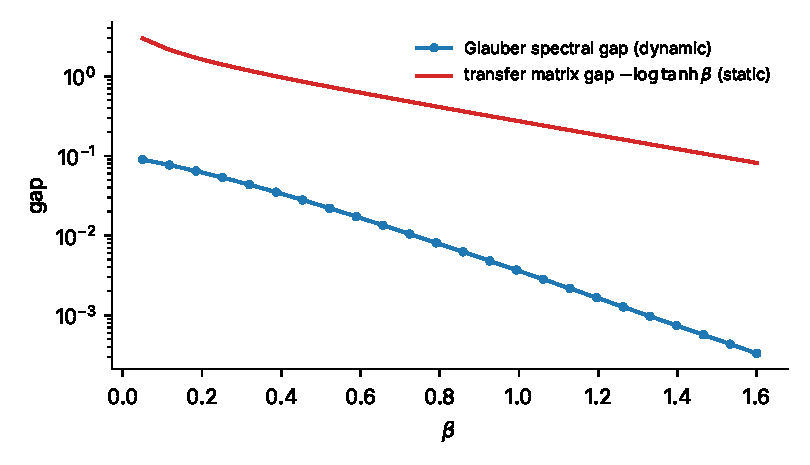
\includegraphics[width=0.85\textwidth]{figures/dynamic_static_gap.pdf}
\caption[Dynamic and static gaps for the Ising chain]{Spectral gap of heat bath Glauber dynamics on a ten site Ising ring, computed exactly, and the transfer matrix gap $-\log\tanh\beta$. Both shrink as the correlation length grows.}
\label{fig:dynstat}
\end{figure}

\subsection{The equivalence theorems}

For finite range spin systems with a finite (discrete) single spin space the following are equivalent, under mild conditions on the boundary behaviour. This is the setting of the theorems quoted below. Lattice Yang Mills has compact continuous spins and a gauge symmetry, so these equivalences are not established for it in this form, and here they serve as a guide.
\begin{enumerate}
\item[(a)] Strong spatial mixing: the influence of a boundary condition decays exponentially with distance, uniformly in the volume and the boundary.
\item[(b)] The Glauber dynamics has a spectral gap bounded below uniformly in the volume.
\item[(c)] The Glauber dynamics has a logarithmic Sobolev constant bounded below uniformly in the volume.
\end{enumerate}
Dobrushin and Shlosman~\cite{DS85,DS87} introduced complete analyticity conditions that imply (a). Stroock and Zegarlinski~\cite{SZ92} proved that (c) is equivalent to Dobrushin and Shlosman complete analyticity, which is slightly stronger than (a) as stated, and Martinelli and Olivieri~\cite{MO94} extended the equivalences to the weaker regime of strong mixing for regular volumes.

\subsection{Curvature and log Sobolev}

The Bakry \'Emery criterion~\cite{BE} gives a direct way to prove (c). If the measure has density $e^{-V}$ on a Riemannian manifold with $\mathrm{Ric}+\nabla^2V\ge\kappa>0$, then it satisfies a logarithmic Sobolev inequality with constant $\kappa$. For lattice gauge theory the manifold is a product of copies of the group, whose Ricci curvature is positive, and $V=\beta S$. At small $\beta$ the Hessian of $\beta S$ is a small perturbation of the positive group curvature, and the criterion applies uniformly in the volume.

This is the route of Shen, Zhu and Zhu~\cite{SZZ}. They studied the Langevin dynamics of lattice Yang Mills at strong coupling in any dimension, proved Poincar\'e and log Sobolev inequalities uniformly in the volume when $\beta$ is below an explicit threshold, and deduced exponential ergodicity, factorisation of Wilson loop correlations at large $N$, and a positive mass gap for the infinite volume measure. Their threshold, of order $1/(16(d-1))$ for SU(N) in their scaling, is a strong coupling condition, in the same regime as the Osterwalder and Seiler cluster expansion~\cite{OSe}, but the proof is entirely through dynamics and curvature.

\subsection{A dynamic route along the ladder}

At weak coupling the Hessian of $\beta S$ is large and indefinite on the scale of the group, and the Bakry \'Emery criterion fails, as it must: the correlation length in lattice units diverges and no dynamic gap uniform in the coupling can exist on the original lattice (at fixed coupling a gap uniform in the volume is expected). The renormalization group suggests a fix. Along the Migdal Kadanoff ladder, every rung is a lattice theory at an effective coupling that decreases by about $\frac34\E S_{\mathrm{BPY}}=\frac14$ per step at leading order (Remark~\ref{prop:decrementB}), until the coupling is below the strong coupling threshold. On that final rung the Shen, Zhu and Zhu argument gives a uniform log Sobolev inequality and hence a gap, provided it applies to the non Wilson plaquette law of that rung, which has not been checked here (their argument is for the Wilson action). The gap of the original theory in physical units then follows if the comparison between rungs preserves log Sobolev constants up to the rescaling of lengths.

That is a dynamic version of the Thorin sandwich of Chapter~\ref{ch:sandwich}: instead of bracketing spectral measures, bracket Dirichlet forms. Comparisons of Dirichlet forms are a standard tool in Markov chain theory, but whether they behave well under the two operations of the ladder is open. The bond moving step multiplies densities on the same group ($f\mapsto f^4$), so it does not produce a product measure on a product space and tensorisation of log Sobolev constants does not apply to it; under such pointwise reweighting the constants are controlled only by perturbation bounds that degrade with the oscillation of $\log f^4$. For convolution with a heat kernel the control by Bakry \'Emery calculus on the group has not been worked out here. The open question is the same as before, the comparison between the ladder and the true lattice, but in a language where more tools are available.

\section{The Renormalization Group for Statisticians}\label{ch:rg}\index{renormalization group}\index{hierarchical lattice}\index{Gaussian ledger}

The renormalization group is the central idea of modern statistical physics, and it is close in spirit to ideas statisticians use every day: hierarchical models, sufficient reductions, and the propagation of uncertainty through levels. This section explains it in that language, with the Migdal Kadanoff ladder as the running example.

\subsection{Coarse graining as marginalisation}

Start with a probability model for fine scale variables, the spins or links of a lattice. Group them into blocks and define a block variable for each, such as a majority vote or an average. The law of the block variables is a marginal of the original law. If it has the same form as the original, with changed parameters, we have a map on parameters, the renormalization map. Iterating it describes the model at larger and larger scales.

In Bayesian terms, the fine variables are latent, the block variables are a coarse summary, and the renormalization map is the update of the hyperparameters that describe the summary. The question the renormalization group asks is what happens to those hyperparameters after many levels. Most hyperparameters become irrelevant: their influence on the coarse law decays. A few are relevant or marginal and determine the large scale behaviour.

\subsection{Fixed points and flows}

A fixed point of the renormalization map is a model that looks the same at every scale. Near a fixed point the map is approximately linear, and its eigenvalues classify directions as relevant, growing under the flow; irrelevant, shrinking; or marginal, neither at linear order. Critical points of statistical models sit on the stable manifolds of nontrivial fixed points, and the exponents of correlation functions are read off from the eigenvalues.

For Yang Mills the relevant picture has two fixed points: the free theory at $g=0$, which is the ultraviolet fixed point, and a strong coupling, confining regime that acts as an infrared attractor. The coupling is marginal at the free fixed point, and its slow logarithmic flow away from it is asymptotic freedom. The continuum limit is the renormalized trajectory that leaves the free fixed point, and the mass gap is the statement that this trajectory ends in the confining regime with a finite correlation length in physical units.

\subsection{Exact renormalization: chains and hierarchical models}

The Ising chain has an exact renormalization map, $\tanh K'=(\tanh K)^2$, from Section~\ref{ch:examples}. Every coupling flows to zero, the disordered fixed point, and the correlation length halves at each step. Two dimensional lattice gauge theory has the same structure, with character coefficients raised to the power $b^2$.

Dyson~\cite{Dy69} introduced hierarchical models, in which the interaction between two spins depends on the level of the smallest block containing both. Their renormalization map is exact by construction, and Bleher and Sinai~\cite{BS73} used them to study critical behaviour rigorously. Migdal Kadanoff lattices, built by repeatedly replacing a bond by a diamond of bonds, are hierarchical lattices on which the Migdal Kadanoff recursion is exact. For spin models that is the diamond construction; a gauge theory needs a plaquette complex, and the gauge version is the one of~\cite{Ito85}. If the gauge recursion of Sections~\ref{ch:mk} and~\ref{ch:verification} is accepted as the exact renormalization of that model, as taken from~\cite{Ito85} and not reproved here, then the ladder is a statement about a real statistical model, the gauge theory on a hierarchical lattice, as well as an approximation to the theory on $\Z^4$.

\subsection{The Gaussian ledger, again}

For Gaussian models the renormalization map is linear algebra. The ledger of Section~\ref{ch:mk}, precisions add under products and variances add under convolutions, makes the four dimensional coupling exactly marginal in flat space. Figure~\ref{fig:ledger} illustrates the consequence, schematically: in flat space the coupling stays where it starts; on the curved group it decreases by a fixed amount per step until strong coupling takes over and it collapses.

\begin{figure}[t]
\centering
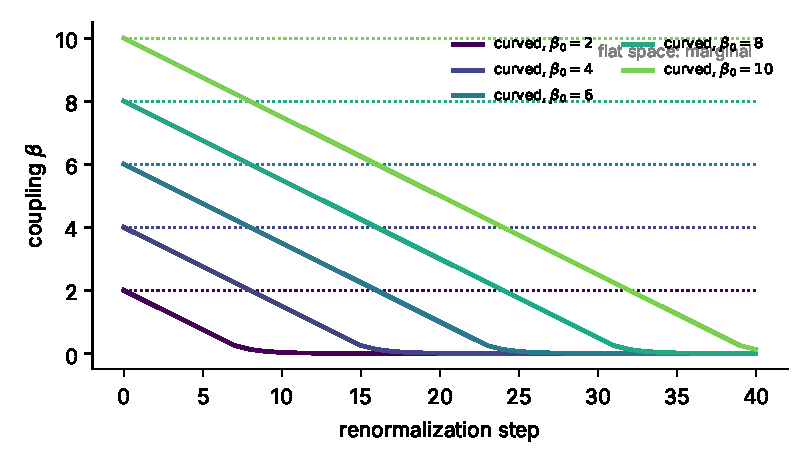
\includegraphics[width=0.85\textwidth]{figures/gaussian_ledger.pdf}
\caption[The Gaussian ledger in flat and curved space]{Schematic renormalization flow of the coupling. Dotted: flat space, where the four dimensional coupling is marginal. Solid: the curved group, where each step lowers the coupling by about $1/4$ until the strong coupling region is reached.}
\label{fig:ledger}
\end{figure}

\subsection{The flow in the space of plaquette laws}

The Migdal Kadanoff map acts on whole plaquette laws, not just one coupling. Figure~\ref{fig:mkphase} projects the flow onto the first two Thorin levels $(u_2,u_3)$. Numerically, trajectories started at weak and intermediate coupling ($\beta_0=3,5,8,12$) lock onto a single curve toward the origin, the heat kernel family $u_3=u_2^{8/3}$. This is a numerical observation, not a theorem, and it is restricted to weak and intermediate coupling: near the origin every trajectory leaves the curve (at strong coupling the character expansion gives $u_3\sim c\,u_2^2$, not $u_2^{8/3}$), and a trajectory started at $\beta_0=0.8$ never reaches it. On linear axes the departure is invisible because $u_3$ is tiny. So the heat kernel laws attract the flow only in that range, and that is the only statistical justification offered for the one dimensional projection used in Section~\ref{ch:verification}.

\begin{figure}[t]
\centering
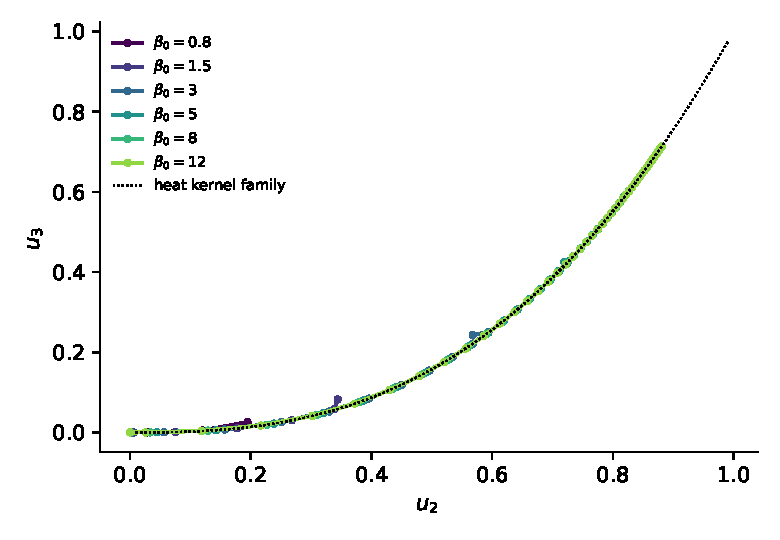
\includegraphics[width=0.85\textwidth]{figures/mk_phase.pdf}
\caption[The Migdal Kadanoff flow in the plane of Thorin levels]{Migdal Kadanoff trajectories for SU(2) projected onto $(u_2,u_3)$, from several Wilson starting couplings. Started at weak and intermediate coupling they follow the heat kernel family $u_3=u_2^{8/3}$, shown dotted (numerical observation); near the origin they leave it.}
\label{fig:mkphase}
\end{figure}

\subsection{Renormalization and hierarchical Bayes}

The analogy with hierarchical Bayesian models runs deep. A hierarchical model with many levels, each level a convolution of the one below with a prior and a product with the data at that level, is a renormalization group in reverse: information flows from coarse to fine. Shrinkage priors such as the horseshoe have a scale mixture structure in which the local scales play the role of irrelevant variables and the global scale the role of a marginal coupling, and the behaviour of the global scale across levels is the statistical analogue of the running coupling. Polson and Scott's duality between envelopes and mixtures~\cite{PSdual} is the bookkeeping of products and convolutions that the Migdal Kadanoff step uses.

\section{Free Fields and Exact Spectral Measures}\label{ch:freefield}\index{free field}\index{K\"all\'en Lehmann representation}

Before an interacting theory, a free one. A free massive field has a gap equal to its mass, and every spectral measure of its local observables is explicit. This section computes them, shows how Routes A and B look when everything is known, and explains which features of the free field survive in Yang Mills and which do not.

\subsection{The K\"all\'en Lehmann representation}

For a free scalar field of mass $m$ in $d$ spacetime dimensions, the zero momentum correlation of the field itself is a single exponential, $C(\tau)\propto e^{-m\tau}$, with spectral measure a point mass at $m$. Composite operators have continuous spectra. The operator $\phi^2$ at zero spatial momentum creates pairs of particles with momenta $p$ and $-p$, of total energy $E=2\sqrt{m^2+p^2}$. Counting states in $d-1$ spatial dimensions and including the normalisation $1/(2\omega)^2$ of each pair gives the spectral density
\[
\rho(E)\propto\frac{(E^2/4-m^2)^{(d-3)/2}}{E},\qquad E>2m .
\]
In two dimensions the density has an inverse square root singularity at threshold; in three it jumps to a constant times $1/E$; in four it rises from zero like a square root (Figure~\ref{fig:ff}). In all cases the support starts at $2m$, so the gap of $\phi^2$ is $2m$, twice the gap of $\phi$. The gap of the theory is the infimum over observables, $m$.

\begin{figure}[t]
\centering
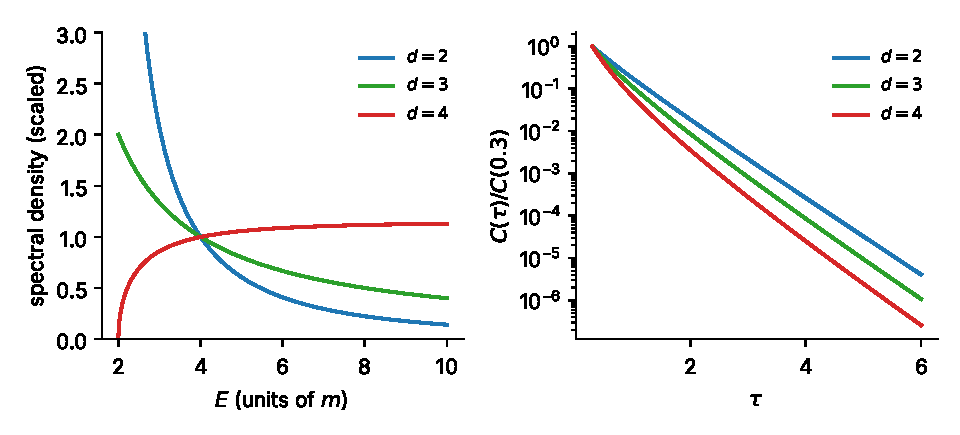
\includegraphics[width=\textwidth]{figures/free_field_kl.pdf}
\caption[Spectral densities of $\phi^2$ for a free field]{Left: zero momentum spectral densities of $\phi^2$ for a free field of mass one in $d=2,3,4$. Right: the corresponding Euclidean correlations, normalised at $\tau=0.3$; all decay at rate $2m=2$, with a power law prefactor set by the threshold behaviour.}
\label{fig:ff}
\end{figure}

\subsection{Routes A and B for a free field}

For the elementary field, Route A gives a gamma variable with rate $m$, and Route B a single damped oscillation in real time. For $\phi^2$, Route A gives a GGC with a continuous Thorin density supported on $[2m,\infty)$, and its tail is expected to be $e^{-2mx}$ times a power determined by the threshold exponent $(d-3)/2$ (a Tauberian computation left to the exercises and not carried out here). Route B gives Thorin densities $T_\alpha(z)$ whose decay rate in $\alpha$ is $2m$ and whose dependence on real time reflects the shape of the density at threshold.

Figure~\ref{fig:thorinheat} shows a Route B Thorin density as a colour map in Euclidean and real time, for the toy glueball spectrum of earlier chapters. The density decays along the Euclidean axis at the gap and oscillates along the real time axis at the frequencies of the stable states, with the continuum smoothing the oscillations at large real time.

\begin{figure}[t]
\centering
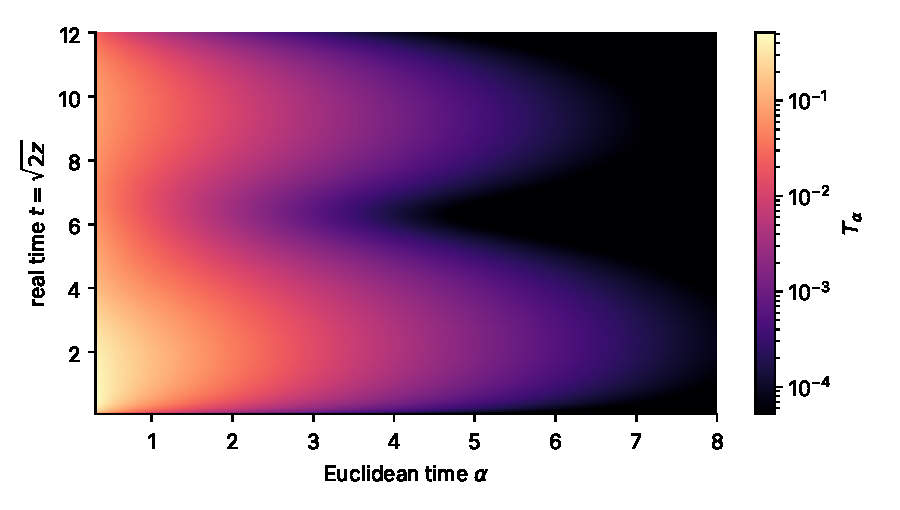
\includegraphics[width=\textwidth]{figures/thorin_heatmap.pdf}
\caption[A Route B Thorin density as a colour map]{The Route B Thorin density $T_\alpha$ for the toy glueball spectrum, as a function of Euclidean time $\alpha$ and real time $y=\sqrt{2z}$, on a logarithmic colour scale. Decay along $\alpha$ is set by the gap; oscillation along $y$ by the stable states.}
\label{fig:thorinheat}
\end{figure}

\subsection{What survives in Yang Mills}

Three features of the free field carry over. The gap of the theory is the infimum over observables, and composite observables have continuous spectra above multiparticle thresholds. Ultraviolet divergences of composite operators, visible here as the failure of $\rho(E)$ to decay at large $E$ in four dimensions, require the offset of Chapter~\ref{ch:positivity}. And the Thorin structure is the same: positive spectral measures, Routes A and B, the equivalence theorem.

Two features do not survive. In Yang Mills there is no elementary field whose spectral measure is a single atom: gauge invariant observables are composite, and the lightest state is expected, on lattice evidence, to be a bound state, the scalar glueball (its mass is a lattice Monte Carlo estimate~\cite{Te98,MP}, not an established fact), whose mass is not a parameter of the Lagrangian but is generated dynamically as a multiple of $\Lambda$. And the free field has a gap because its mass is put in by hand. The entire difficulty of the Clay problem is that Yang Mills has no mass term, and the gap must be produced by the renormalization group flow from the massless free fixed point. A free massive field is the answer we expect the long distance limit to resemble, not a step on the way to proving it.

\section{Large N and Free Probability}\label{ch:largeN}\index{large $N$}\index{Gross Witten Wadia transition}\index{free probability}

't Hooft~\cite{tH74} observed in 1974 that SU(N) gauge theory simplifies as $N\to\infty$ with $\lambda=g^2N$ fixed: only planar diagrams survive, and the theory becomes a theory of strings. Large $N$ is where gauge theory meets random matrix theory and free probability, both close to the probabilistic toolkit of this book. This section explains what large $N$ says about the gap.

\subsection{The Gross Witten Wadia transition}

The simplest large $N$ lattice gauge theory is a single plaquette, or equivalently two dimensional lattice gauge theory, with weight $\exp(\frac N\lambda\operatorname{tr}(U+U^\dagger))$ on a single unitary matrix. Gross and Witten~\cite{GW80}, and independently Wadia, solved it at large $N$. The eigenvalue angles $\theta\in(-\pi,\pi]$ of $U$ have a limiting density that changes form at $\lambda=2$:
\[
\rho(\theta)=\begin{cases}\dfrac{2}{\pi\lambda}\cos\dfrac\theta2\sqrt{\dfrac\lambda2-\sin^2\dfrac\theta2}, & \lambda<2,\\[1.2em] \dfrac{1}{2\pi}\Big(1+\dfrac2\lambda\cos\theta\Big), & \lambda\ge2 .\end{cases}
\]
At weak coupling the eigenvalues are confined to an arc and the density has a gap on the circle; at strong coupling they cover the whole circle (Figure~\ref{fig:gww}). The free energy is analytic on each side but its third derivative jumps at $\lambda=2$: a third order phase transition, which exists only at infinite $N$.

\begin{figure}[t]
\centering
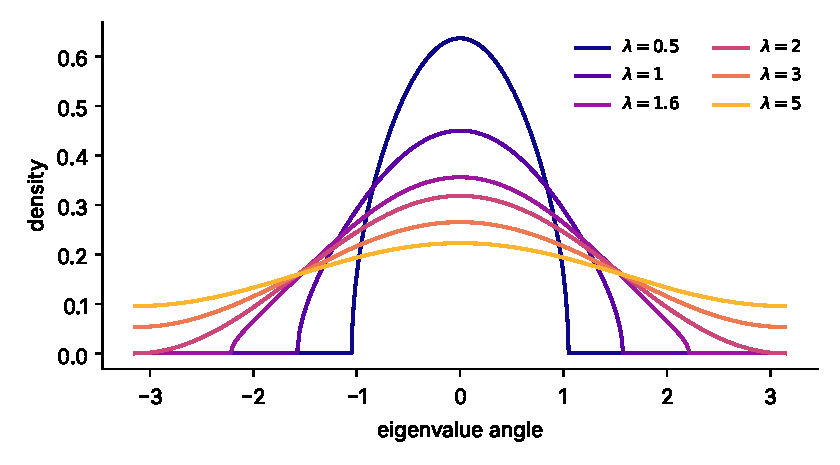
\includegraphics[width=0.85\textwidth]{figures/gww.pdf}
\caption[Gross Witten Wadia eigenvalue densities]{Limiting eigenvalue densities of the Gross Witten Wadia model for several values of $\lambda$. Below $\lambda=2$ the support is an arc; above, the whole circle.}
\label{fig:gww}
\end{figure}

Douglas and Kazakov~\cite{DK} found the analogous transition in continuum two dimensional Yang Mills on the sphere, at a critical area. In both cases the transition separates a weak coupling phase, dominated by small fluctuations around the identity, from a strong coupling phase, dominated by disordered eigenvalues.

\subsection{Free Brownian motion on the unitary group}

As $N\to\infty$, Brownian motion on U(N) has a limit in the sense of free probability: the eigenvalue distribution at time $t$ converges to a deterministic law on the circle, the law of Biane's free unitary Brownian motion~\cite{Bi97}. For small $t$ the support is an arc that grows with $t$; at $t=4$ it closes up and covers the circle. Two dimensional Yang Mills at large $N$ is governed by this process, the master field (Levy~\cite{Le17} constructed the master field on the plane as the large $N$ limit of planar Yang Mills holonomies, which satisfies the Makeenko Migdal equations), and the Douglas Kazakov transition is where the free unitary Brownian motion bridge from the identity back to itself can no longer avoid wrapping around the circle.

The three sphere heat kernel of Section~\ref{sec:su2bm}, shown as a colour map in Figure~\ref{fig:hkheat}, is the $N=2$ case of Brownian motion on SU($N$), although Biane's time normalisation differs from the one used for $K_t$. As $N$ grows, the heat kernel on SU(N) concentrates, and its eigenvalue distribution becomes deterministic.

\begin{figure}[t]
\centering
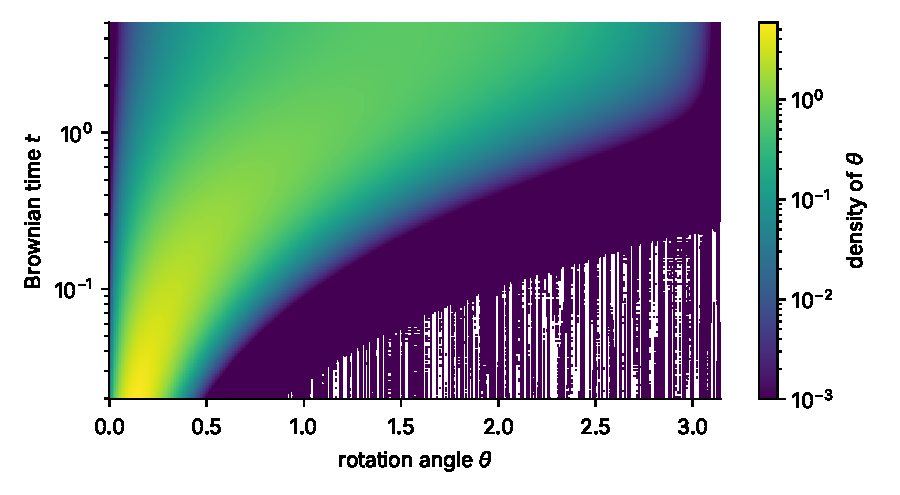
\includegraphics[width=\textwidth]{figures/heat_kernel_heatmap.pdf}
\caption[The SU(2) heat kernel as a colour map]{Density of the rotation angle of Brownian motion on SU(2) as a function of Brownian time, on a logarithmic colour scale. At small times the mass sits near the identity; by $t\approx5$ the law is close to Haar.}
\label{fig:hkheat}
\end{figure}

\subsection{What large N says about the gap}

At large $N$ the glueball masses, in units of the string tension, are expected to have finite limits, and lattice computations indicate that they are close to their $N=3$ values~\cite{Te98}. The large $N$ theory is believed to have a gap, and it is a theory of free glueballs: glueball scattering amplitudes vanish like $1/N^2$. In the language of this book, the spectral measure of a single trace observable at large $N$ is a sum of point masses, the stable glueballs, with no multiparticle continuum at leading order. Route A then gives a convolution of gamma variables, and Route B a sum of damped oscillations.

The large $N$ limit does not make the Clay problem easier in any known way. The master field is understood in two dimensions, where it is free unitary Brownian motion, but not in four. What large $N$ does supply is a family of exactly solvable caricatures in Kac's sense, where the relation between the eigenvalue distribution of the plaquette and the confining behaviour can be studied, and where free probability, a probabilistic theory, is the natural language.

\section*{Exercises}
\begin{enumerate}
\item Derive the eigenvalues $u_n(\beta)^L$ of the two dimensional transfer matrix on a cylinder of $L$ sites by integrating out the links of one time slice.
\item Using Amos's lower bound, show that $\Delta(a)\le\frac{g^2\ell\beta}{4}\operatorname{arcsinh}(2/\beta)$, and find the limit of this upper bound as $a\to0$.
\item Compute the two dimensional Yang Mills partition function on the torus for SU(2) (Section~\ref{sec:su2bm}) as a theta function and use the Jacobi transformation to find its behaviour as $A\to0$.
\item Verify the row $\beta=2$ of the table of Section~\ref{ch:tour}.
\item Show that the Wilson loop of area $A$ in two dimensions is $u_2^A$, and that the potential between static charges is linear at every coupling.
\item Show that the gap ratio $(-\log u_2)/x$ tends to one as $\beta\to\infty$ and to zero as $\beta\to0$.
\item Compute the spectral gap of heat bath dynamics for a single Ising spin in a field.
\item Show that a logarithmic Sobolev inequality implies a Poincar\'e inequality with the same constant.
\item Show that the log Sobolev constant of a product measure on a product space is the minimum of the constants of its factors, and explain why this does not apply to the bond moving step $f\mapsto f^4$ of Section~\ref{ch:dynamic}.
\item Derive the Ising chain renormalization map and its fixed points (Section~\ref{ch:rg}).
\item For a Gaussian free field on $\Z^d$, compute the renormalization of the mass term under block averaging and show it is relevant.
\item Verify that the heat kernel family is invariant under decimation and explain why it is approximately invariant under bond moving at weak coupling.
\item Derive the two particle spectral density of $\phi^2$ in $d$ dimensions.
\item Compute the Route A Thorin measure for $\phi^2$ in two dimensions and its tail.
\item Show that the zero momentum correlation of $\phi^2$ in four dimensions diverges as $\tau\to0$ and find the rate.
\item Verify that both Gross Witten Wadia densities integrate to one and agree at $\lambda=2$.
\item Compute the first moment $\int\cos\theta\,\rho(\theta)\mathrm d\theta$ on each side of the transition and show that it is continuous with a continuous derivative.
\item Explain why the third order transition cannot occur at finite $N$.
\end{enumerate}
